\documentclass[xcolor=dvipsnames]{beamer}  % ALLOWS CHANGE IN COLOR
\usepackage{beamerthemesplit}

%% commenting the above and uncommenting below prints handout (use 4 on 1 or 8 on 1)
% \documentclass[handout,xcolor=dvipsnames]{beamer}     % TO PRINT PRESENTATION HANDOUT
% \usepackage{pgfpages}
% \pgfpagesuselayout{8 on 1}[letter, border shrink=5mm]

\usepackage{url}
\usepackage{ae} % or {zefonts}
\usepackage[T1]{fontenc}
\usepackage[ansinew]{inputenc}
\usepackage[spanish,es-nodecimaldot]{babel}

\usepackage{amsmath}

\usepackage{graphicx}
%\graphicspath{"../../graphs/"}
\usepackage{color}
%\usepackage[colorlinks]{hyperref} % beamer loads this by default, needed only to change default behavior? 
\usepackage{tikz} % Easier syntax to draw pgf files (invokes pgf automatically)
\usetikzlibrary{arrows,shapes.geometric}

\usepackage{tabulary} % automatic column length in tables with long text string
%% use LRJC for auto, and lrjc for normal column width
\setlength\tymin{10pt}       %% change behavior, see p. 254 LaTeX companion
\setlength\tymax{\maxdimen}  %% change behavior, see p. 254 LaTeX companion

\usepackage{multirow} %allows multiple rows in tables

%\usecolortheme{crane}     %Color yellow
%\usetheme{Warsaw}
\usecolortheme[named=Gray]{structure}

\useoutertheme[footline=empty]{}  % PUTS COLORED LINE AT FOOT WITH TITLE, AUTHOR, PAGE, etc
%\usetheme{Berkeley}
\usetheme[height=7mm]{Rochester}
%\setbeamertemplate{items}[ball]   % ITEMS IN 3D BALLS (alt CIRCLES)
\setbeamertemplate{navigation symbols}{}  % DROPS NAVIGATION ICONS
\setbeamertemplate{blocks}[rounded][shadow=true]

%\setbeamertemplate{footline} {
%    \begin{beamercolorbox}{section in head/foot}
%    \insertsectionnavigationhorizontal{\paperwidth}{}{plus1filll
%    \insertframenumber}
%    \end{beamercolorbox}
%}

%\setbeamertemplate{navigation symbols}{\insertslidenavigationsymbol,
%\insertdocnavigationsymbol} \setbeamertemplate{footline} {
%    \begin{beamercolorbox}{section in head/foot}
%    \insertsectionnavigationhorizontal{\paperwidth}{}{plus1filll
%    \insertframenumber}
%    \end{beamercolorbox}
%}

\setbeamercovered{transparent}
\setbeamertemplate{caption}{\insertcaption}
\setbeamertemplate{footline}[frame number] % adds slide number, overrides split footer with authors/title that the theme uses

\tikzstyle{nodo} = [circle, draw=black, fill=white, text=black]
\tikzstyle{end} = [circle, minimum width=3pt,fill, inner sep=0pt]

% \AtBeginSection[] {
%    \begin{frame}
%        \frametitle{Road map}
%        \tableofcontents[currentsection]
%    \end{frame}
% }

\title[Redistricting strategy]{Transparency, automated redistricting, and partisan strategic interaction in Mexico}
%\subtitle{Party bias and responsiveness in Mexico}
\author[Trelles, Altman, Magar, McDonald]{A. Trelles\inst{1} \and M. Altman\inst{2} \and E. Magar\inst{3}  \and M.P. McDonald\inst{4}}
\institute[ITAM-MIT-UFG-Pitt]{\inst{1} Pitt \and
                              \inst{2} MIT \and
                              \inst{3} ITAM \and 
                              \inst{4} UFL}
%\address{}
\date[13may16]{Taller La ciencia pol�tica desde M�xico, ITAM \\ 5/13/16}

\begin{document}

%%%%%%%%%%%%%%%%%%%%%%%%%%%%%%%%%%%%%%%%%%%%%%%%%%%%%%%%%%%%%%%%%%%%%%%%%%%%%%%%%%%%%%%%%%%%

\frame[plain]{\titlepage}

%%%%%%%%%%%%%%%%%%%%%%%%%%%%%%%%%%%%%%%%%%%%%%%%%%%%%%%%%%%%%%%%%%%%%%%%%%%%%%%%%%%%%%%%%%%%
\begin{frame}                      % SLIDE

    \frametitle{Motivation}

Redistricting by independent commission

\begin{enumerate}
\item Taking politicians out of map drawing ensures a fair result?
\item Can parties influence district boundaries? How?
\item How can the redistricting process be made more transparent?
\end{enumerate}

\bigskip

Paper inspects the case of Mexico since 1997


\end{frame}
%%%%%%%%%%%%%%%%%%%%%%%%%%%%%%%%%%%%%%%%%%%%%%%%%%%%%%%%%%%%%%%%%%%%%%%%%%%%%%%%%%%%%%%%%%%%%%%%
% \frame {                      % SLIDE
%     \frametitle{Road map}
% \tableofcontents%[section=1]
% }
%%%%%%%%%%%%%%%%%%%%%%%%%%%%%%%%%%%%%%%%%%%%%%%%%%%%%%%%%%%%%%%%%%%%%%%%%%%%%%%%%%%%%%%%%%%%%%%%
\section{Redistricting in Mexico}
%%%%%%%%%%%%%%%%%%%%%%%%%%%%%%%%%%%%%%%%%%%%%%%%%%%%%%%%%%%%%%%%%%%%%%%%%%%%%%%%%%%%%%%%%%%%%%%%
\begin{frame}                      % SLIDE

    \frametitle{Background on Mexico}

\begin{itemize}

\item 32 states
\item Democratic since 1997
\item Lower chamber of Congress elected every 3 years
\item Mixed system: 300 SMD + 200 PR seats
\item Single-term limits removed in 2018
\item Independent board (IFE) organizes elections and redistricting

\end{itemize}

\end{frame}
%%%%%%%%%%%%%%%%%%%%%%%%%%%%%%%%%%%%%%%%%%%%%%%%%%%%%%%%%%%%%%%%%%%%%%%%%%%%%%%%%%%%%%%%%%%% 

\begin{frame}                      % SLIDE
    \frametitle{The redistricting process}
\begin{center}
   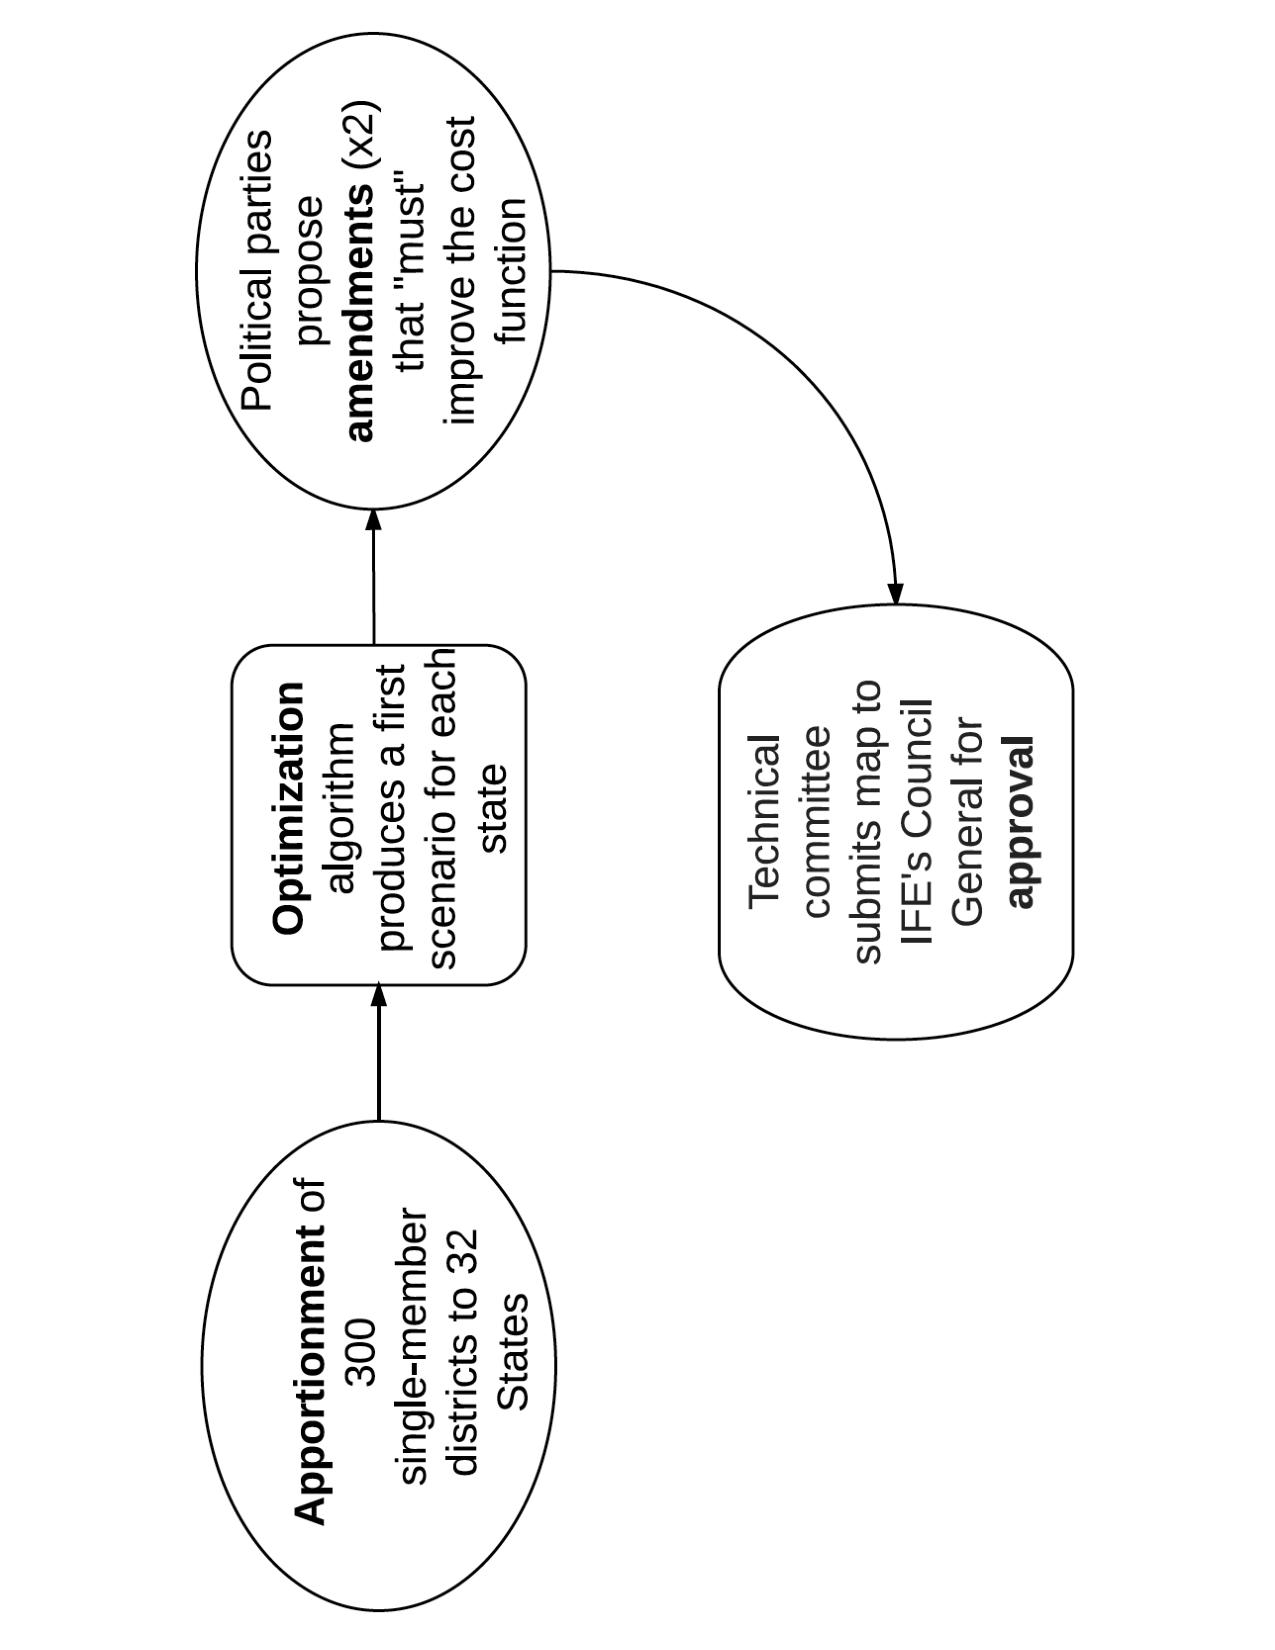
\includegraphics[width=8cm, angle=-90]{../../graphs/mexRedisProcessFlowchart.pdf}
\end{center}

\end{frame}
%%%%%%%%%%%%%%%%%%%%%%%%%%%%%%%%%%%%%%%%%%%%%%%%%%%%%%%%%%%%%%%%%%%%%%%%%%%%%%%%%%%%%%%%%%%% 
\begin{frame}                      % SLIDE
    \frametitle{Apportionment}


Hamilton method used:

\begin{itemize}
\item The quota (or price of a seat) is $Q = \frac{\text{nation's population}}{300}$

\item First allocation is $\frac{\text{state's population}}{Q}$, rounded down

\item Every state gets 2 seats min

\item Unallocated seats, if any, awarded to states with largest fractional remainders
\end{itemize}

\bigskip

%\pause

Most recent decennial census must be used 

\begin{itemize}
\item ... but no obligation to redistrict as soon as available
\item 7-year lag on average: 199\textbf{7}, 200\textbf{6}, 201\textbf{8}
%\item and IFE considers $\pm15\%$ imbalance normal (!)
\end{itemize}

\bigskip

Bureaucratic leeway: $\pm15\%$ tolerance

\end{frame}
% %%%%%%%%%%%%%%%%%%%%%%%%%%%%%%%%%%%%%%%%%%%%%%%%%%%%%%%%%%%%%%%%%%%%%%%%%%%%%%%%%%%%%%%%%%%% 
% \frame{                      % SLIDE
%     \frametitle{District populations: linear projection}

% \centering

% 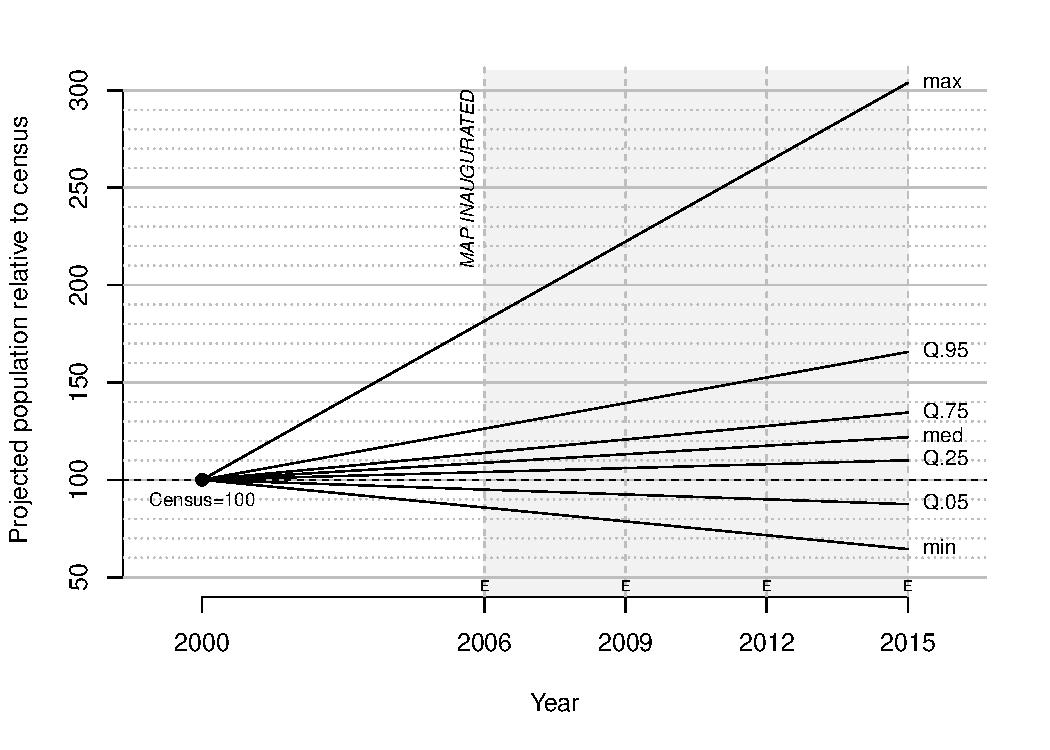
\includegraphics[width=.99\textwidth]{../../graphs/disRelPopProj2006map.pdf}

% %\pause

% Plus: bureaucratic leeway in new district sizes %$\rightarrow$ substantial malapportionment


% }
%%%%%%%%%%%%%%%%%%%%%%%%%%%%%%%%%%%%%%%%%%%%%%%%%%%%%%%%%%%%%%%%%%%%%%%%%%%%%%%%%%%%%%%%%%%% 
\frame{                      % SLIDE
    \frametitle{Malapportionment is substantial}

\centering

%$RRI = \frac{1/\text{district size}}{300/\text{national population}} = \frac{Q}{\text{district size}}$
$RRI = \frac{nat. pop./300}{\text{district size}}$

\bigskip

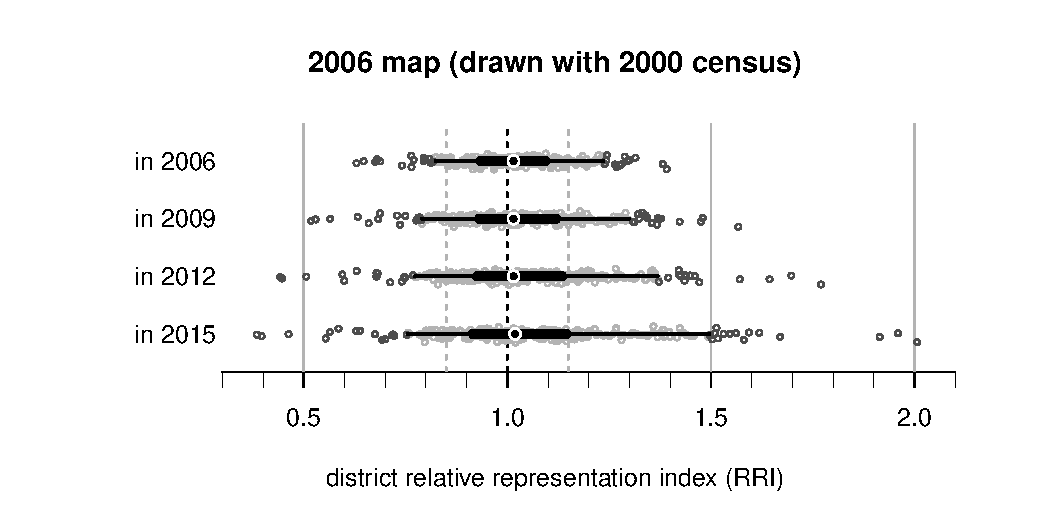
\includegraphics[width=.6\textwidth]{../../graphs/rrin0615d0.pdf} \\
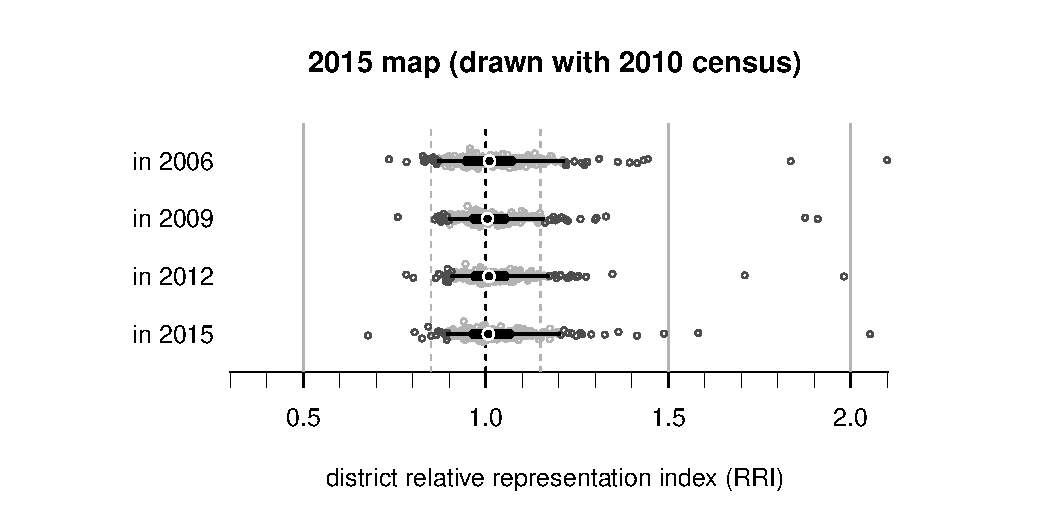
\includegraphics[width=.6\textwidth]{../../graphs/rrin0615d3.pdf} 


}
%%%%%%%%%%%%%%%%%%%%%%%%%%%%%%%%%%%%%%%%%%%%%%%%%%%%%%%%%%%%%%%%%%%%%%%%%%%%%%%%%%%%%%%%%%%% 

\begin{frame}                      % SLIDE

    \frametitle{Automated redistricting}

Redistricting by experts since 1997

\begin{enumerate}
\item no district crosses state boundaries
\item optimization algorithm $\rightarrow$ proposal
\item parties propose amendments (``must'' improve score)
\item repeat 2 and 3 once
\item board approves new map
\end{enumerate}

\begin{multline*}
\texttt{Score} = .4 \times \texttt{PopBalance} + .3 \times \texttt{MunicBoundaries} \\
+ .2 \times \texttt{TravelTime} + .1 \times \texttt{Compactness}
\end{multline*}

%\pause

$\pm15\%$ imbalance considered legal (!)

%Salience should go up: single-term limits dropped in 2018

\end{frame}
% %%%%%%%%%%%%%%%%%%%%%%%%%%%%%%%%%%%%%%%%%%%%%%%%%%%%%%%%%%%%%%%%%%%%%%%%%%%%%%%%%%%%%%%%%%%% 

% \begin{frame}                      % SLIDE
%     \frametitle{Optimization algorithm}

% Simulated annealing = probabilistic meta-heuristic for optimization \\ locates a good approximation to the global optimum of the cost function in a large search space

% \bigskip

% Thousands of iterations using electoral \emph{secciones} 

% \bigskip

% Combinatorial optimization algorithm used to generate 
% the first scenario in each state


% \begin{center}
%    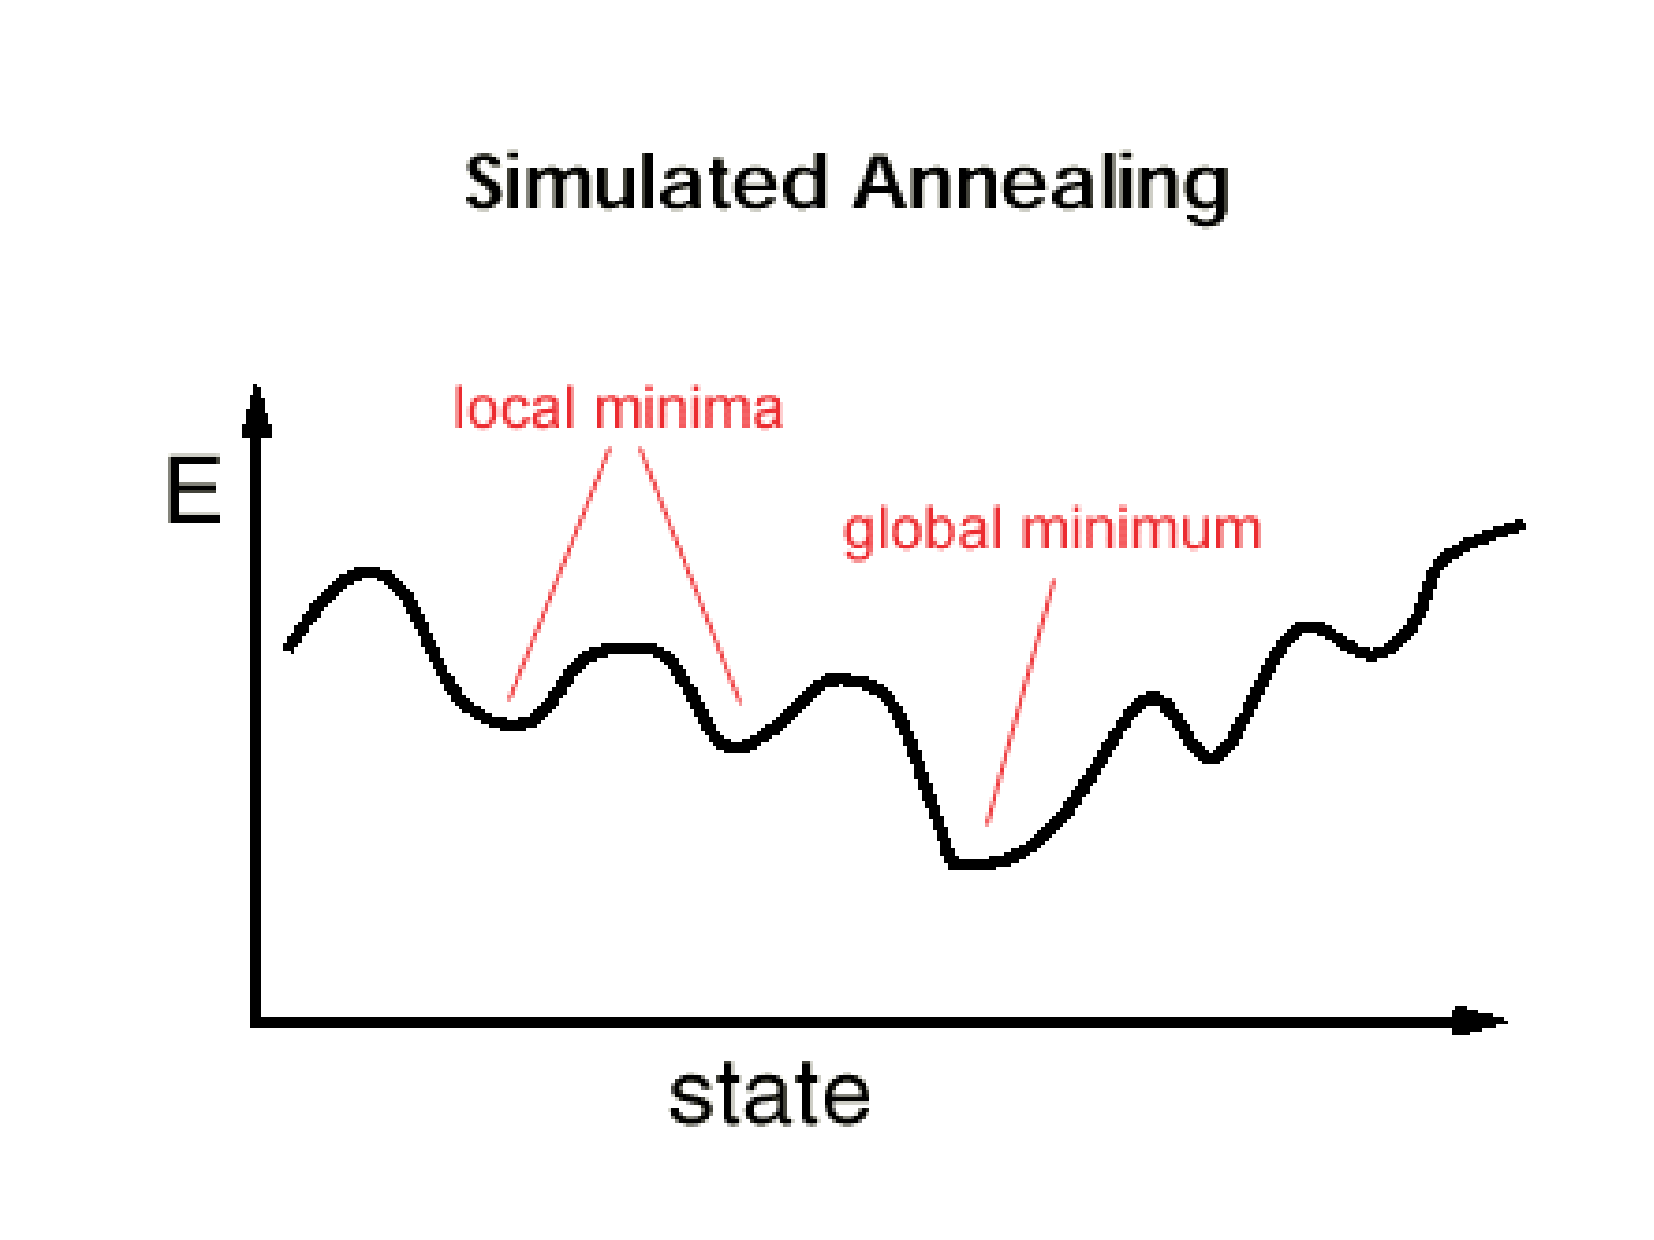
\includegraphics[width=5cm]{../../graphs/sim.pdf}
% \end{center}

% Board claims that this is a public process, but the \\ operation and procedures are done \alert{behind closed doors}

% \end{frame}
%%%%%%%%%%%%%%%%%%%%%%%%%%%%%%%%%%%%%%%%%%%%%%%%%%%%%%%%%%%%%%%%%%%%%%%%%%%%%%%%%%%%%%%%%%%% 
\begin{frame}                                       % SLIDE

    \frametitle{Party amendments}
\begin{center}
   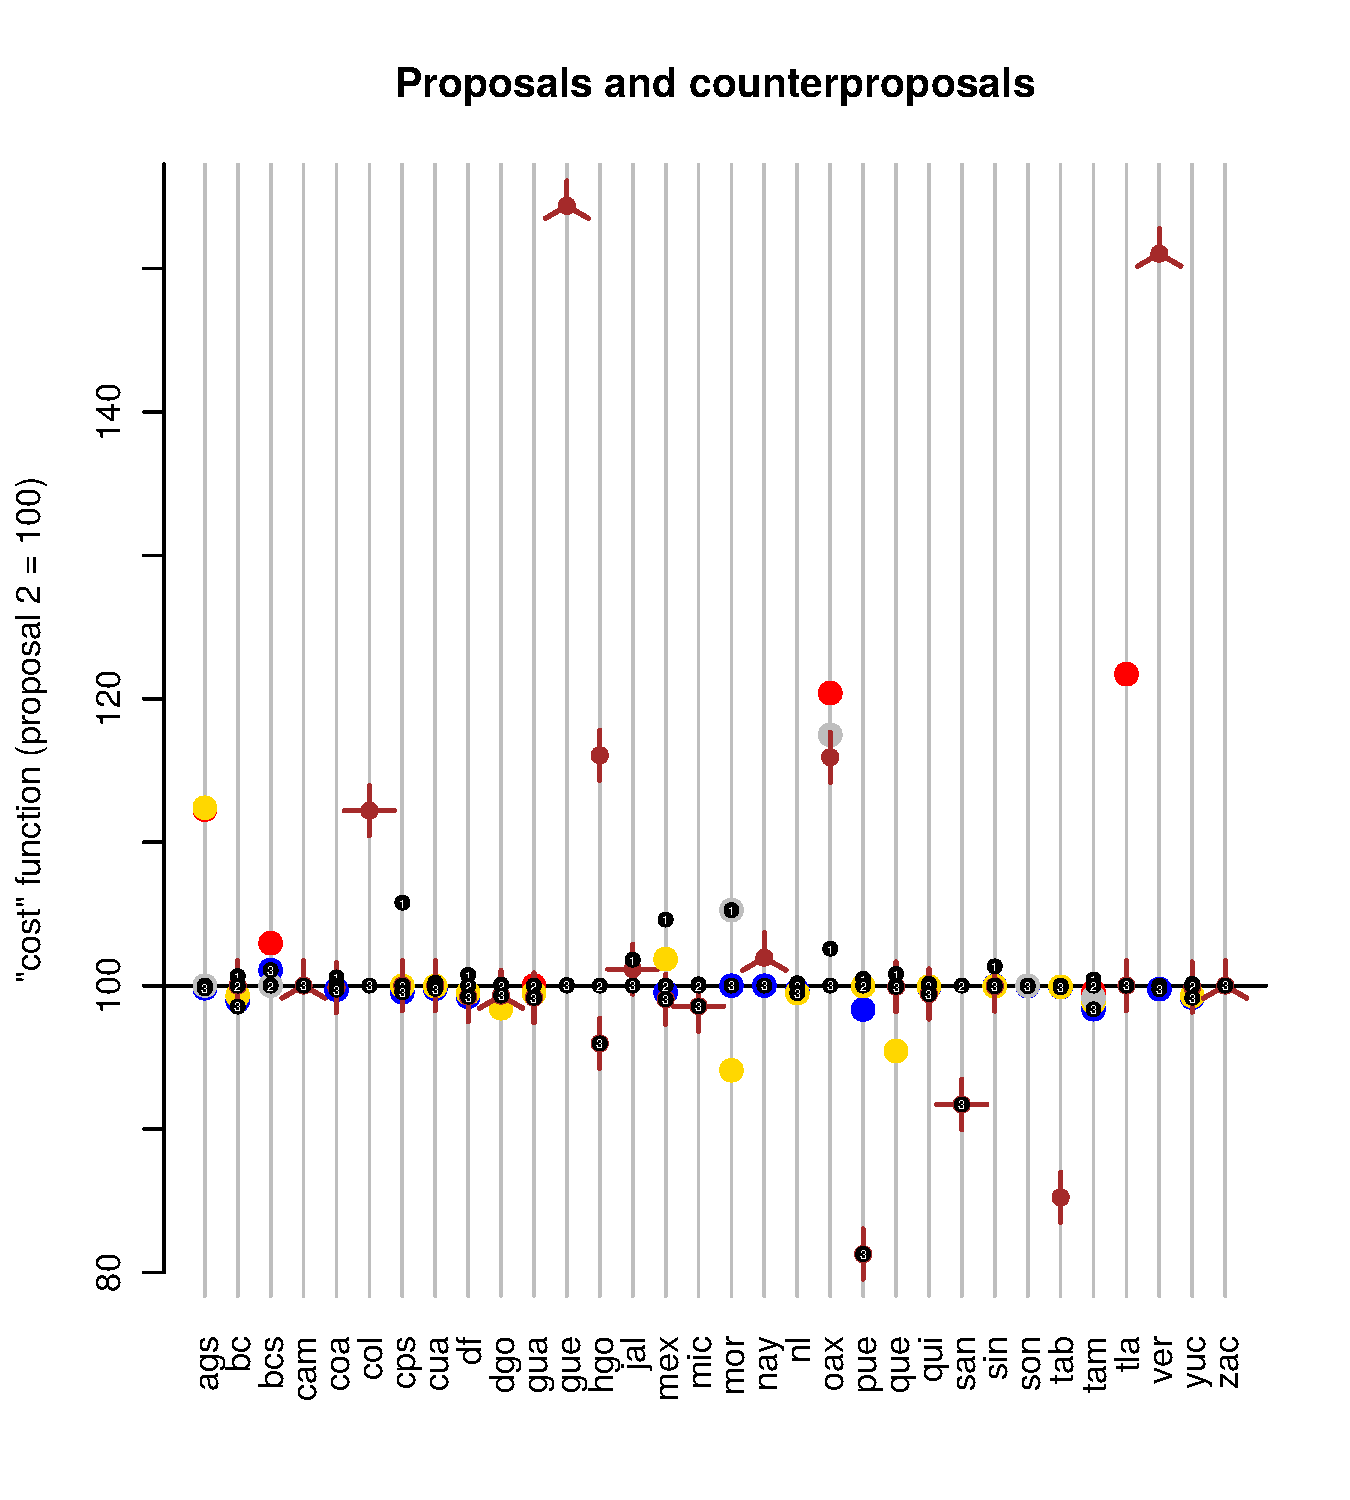
\includegraphics[width=8cm]{../../graphs/propsAndCost.pdf}
\end{center}
\end{frame}
% %%%%%%%%%%%%%%%%%%%%%%%%%%%%%%%%%%%%%%%%%%%%%%%%%%%%%%%%%%%%%%%%%%%%%%%%%%%%%%%%%%%%%%%%%%%% 
% \begin{frame}                                       % SLIDE

%     \frametitle{Party amendments}
% \begin{itemize}
% %\item Humans can beat the computer $\rightarrow$ enables manipulation 
% \item Smoking gun: four maps improved score but \alert{not} adopted
% \item Unobserved: maps improving score but hurting parties?
% \item Asymmetric party capacity to produce counterproposals: by far, PAN most effective. Benefits?
% \item Increased similarity of final map to status quo: parties protecting strongholds?
% %\item Party learning process 
% \end{itemize} 

% \end{frame}


% %%%%%%%%%%%%%%%%%%%%%%%%%%%%%%%%%%%%%%%%%%%%%%%%%%%%%%%%%%%%%%%%%%%%%%%%%%%%%%%%%%%%%%%%%%%% 
\begin{frame}
    \frametitle{Parties protect strongholds?}

District similarity index = share common population \\ (Cox\&Katz 2002)

\bigskip

\begin{center}
\begin{footnotesize}
  \begin{tabular}{lrrrrr}
  Similarity between          &   min  &  25\%  & median &  75\% &  max \\ \hline
  initial proposal and SQ     & 0.128  & 0.419  & 0.584  & 0.755 &  1   \\
  final proposal and SQ       & 0.125  & 0.437  & 0.643  & 0.805 &  1   \\
  final and initial proposals & 0.174  & 0.705  & 0.967  & 1     &  1   \\
  \end{tabular}
\end{footnotesize}
\end{center}
\end{frame}
% %%%%%%%%%%%%%%%%%%%%%%%%%%%%%%%%%%%%%%%%%%%%%%%%%%%%%%%%%%%%%%%%%%%%%%%%%%%%%%%%%%%%%%%%%%%% 
% \begin{frame}\label{fr:MxMapProj}                      % SLIDE

%     \frametitle{The bigger project}

% \emph{Draw Mexico} project = offspring of \emph{Public Mapping Project in U.S.}

% \bigskip

% Remove opaqueness from redistricting process 

% \bigskip

% \texttt{DistrictBuilder} is open-source, web-based software %({\footnotesize \url{www.districtbuilder.org}}):

% \begin{itemize}

% \item enables widespread DIY redistricting thru cloud computing

% \item  internet lets anyone draw/inspect maps: crowdsourcing

% \item redistricting contests in 6 US states $\rightarrow$ hundreds of legal plans

% \end{itemize}

% \bigskip

% Application to \alert{Mexico} \href{http://23.21.151.172/}{\beamergotobutton{Link: MexDemo}} (Donations anyone?) 

% \end{frame}
%%%%%%%%%%%%%%%%%%%%%%%%%%%%%%%%%%%%%%%%%%%%%%%%%%%%%%%%%%%%%%%%%%%%%%%%%%%%%%%%%%%%%%%%%%%%
\frame {                      % SLIDE

    \frametitle{Wrap-up}

\begin{itemize}
\item Transparency in commission's work is a must for accountability
\item Mexico case study:
  \begin{enumerate}
  \item Explicit rules violated
  \item Ad-hoc operationalization
  \item Parties acting as if implicit rules operational
  \end{enumerate}
\item None can be assessed from publicly available information
\end{itemize}
\pause

\bigskip

\begin{center}
\textbf{Thank you!}
\end{center}
}
\end{document}

